% 'draft' mode can be used to speed up compilation
\documentclass[twoside,final]{hcmut-report}
\usepackage{codespace}

% Draft watermark
% https://github.com/callegar/LaTeX-draftwatermark

% Encodings
\usepackage{gensymb,textcomp}

% Better tables
% Wide tables go to https://tex.stackexchange.com/q/332902
\usepackage{array,longtable,multicol,multirow,siunitx,tabularx}

% Better enum
\usepackage{enumitem}

% Graphics
\usepackage{caption}

% Add options for figures, like max width, framing, etc.
\usepackage[export]{adjustbox}

% References
% Use \Cref{} instead of \ref{}
\usepackage[nameinlink]{cleveref}

% FOR DEMONSTRATION PURPOSES, REMOVE IN PRODUCTION
\usepackage{mwe}
%\usepackage{microtype}

\usepackage{amsmath}

\newcommand{\Var}{\text{Var}}
\newcommand{\X}{\mathbf{}{X}}
\newcommand{\A}{\mathbi{A}}
\newcommand{\R}{\mathbb{R}}
\newcommand{\F}{\mathcal{F}}
\newcommand{\N}{\mathbb{N}}
% Sub-preambles
% https://github.com/MartinScharrer/standalone

% Configurations
\coursename{Students-Undergraduate Research Graduate Excellence \\ \href{https://surge.iitk.ac.in/}{(SURGE) Program 2023}}
\reporttype{Project Report}
\title{Stochastic Differential Equations and Applications}
\advisor{& \href{https://www.iitk.ac.in/new/mrinmay-biswas}{Prof. Mrinmay Biswas} \\
         & Department of Mathematics and Statistics, IIT Kanpur \\
         & mbiswas@iitk.ac.in\\
}
\stuname{%
  & Vanshika Gupta \\
  & Department of Mathematics and Statistics \\
  & Institute Roll no. \textbf{211146} \\
  & SURGE Roll no. \textbf{2330436} \\
}

% Allow page breaks inside align* environment
%\allowdisplaybreaks{}

% Makes a lot of things blue, avoid at all costs
%\everymath{\color{blue}}

% Set depth of numbering for counters
\AtBeginDocument{\counterwithin{lstlisting}{section}}

% Rename some sections
%\AtBeginDocument{\renewcommand*{\contentsname}{Contents}}
%\AtBeginDocument{\renewcommand*{\refname}{References}}
%\AtBeginDocument{\renewcommand*{\bibname}{References}}

% Custom commands
%\newcommand*\mean[1]{\bar{#1}}

\begin{document}
\coverpage
%

%\section*{Member list \& Workload}
%\newcounter{memberrowno}
%\setcounter{memberrowno}{0}
%\begin{center}
%  \begin{tabular}{>{\stepcounter{memberrowno}\thememberrowno}llcc}
%    \toprule
%    \multicolumn{1}{c}{\textbf{No.}} & \textbf{Full name} & \textbf{Student ID} & \textbf{Contribution} \\
%    \midrule
%                                     & h                  & xxxxxxx             & 100\%                       \\
%                                     & h                  & xxxxxxx             & 100\%                       \\
%    \bottomrule
%  \end{tabular}
%\end{center}
%\clearpage

\title{\centering \textbf{\underline{CERTIFICATE}}}
\author{}
\date{}

\maketitle

This is to certify that the research project titled \textbf{"Stochastic Differential Equations and Applications"} has been carried out by \textbf{Vanshika Gupta ($2330436$)} under the supervision of \textbf{Prof. Mrinmay Biswas}.The project has been completed in fulfillment of the requirements for the Students-Undergraduate Research Graduate Excellence (SURGE) Program $2023$ offered by Indian Institute of Technology, Kanpur, from $11^{\text{th}}$ May $2023$ to $12^{\text{th}}$ July $2023$. The work presented in this project report is original and has not been submitted elsewhere for any other purpose.

\vspace{5cm}

\begin{flushright}
\textbf{Prof. Mrinmay Biswas}\\
Assistant Professor\\
Department of Mathematics and Statistics\\
Indian Institute of Technology, Kanpur
\end{flushright}


\pagebreak

\maketitle

\begin{center}
\vspace{4cm}
\Large\underline{\textbf{ACKNOWLEDGEMENTS}}
\end{center}
\vspace{2cm}



I would like to express my deepest gratitude to my supervisor, Prof. Mrinmay Biswas, for their unwavering support, guidance, and invaluable expertise throughout the duration of this research project. Their profound knowledge and insightful suggestions have greatly influenced the successful completion of this work.\\
I am thankful to SURGE Program 2023 for their support, which made this research project possible. I would also like to thank the Indian Institute of Technology, Kanpur for providing an environment conducive to research and for their commitment to fostering academic excellence.\\
Lastly, I would like to extend my thanks to my classmates for their assistance and contributions, whether in the form of discussions, resources, or technical support.\\
\vspace{3cm}
\begin{flushright}
    \textbf{Vanshika Gupta}
\end{flushright}


\pagebreak

\begin{center}
\vspace{4cm}
\Large\underline{\textbf{ABSTRACT}}
\end{center}


Stochastic differential equations (SDEs) are powerful mathematical tools for modeling and analyzing dynamic systems affected by random fluctuations. In this research project titled "Stochastic Differential Equations and Applications," we delve into the fundamental concepts, properties, and applications of SDEs.\\
The project begins by establishing the mathematical foundations of SDEs, including probability spaces, random variables, stochastic processes, and the construction of Brownian motion. We explore the theory of stochastic integrals, focusing on the Wiener integral and the Itô integral, which are key tools for solving SDEs.\\
The project investigates the properties of SDEs and their solutions, introducing the concept of a solution to an SDE and discussing the existence and uniqueness theorems. Various numerical schemes, such as Euler's scheme and Euler-Maruyama scheme, are presented as practical methods for approximating the solutions of SDEs.\\
Furthermore, we highlight the applications of SDEs in finance, particularly in modeling stock prices and options pricing. These examples demonstrate how SDEs can capture the inherent uncertainties and complex dynamics of financial markets.\\
Through this project, we aim to deepen our understanding of the underlying stochastic processes that govern dynamic systems and to showcase the practical implications of SDEs in various fields. The insights gained from this study can enhance our ability to make accurate predictions, assess risks, and make informed decisions in the presence of uncertainties.\\
The project report provides a comprehensive overview of the key concepts and results related to SDEs, offering a solid foundation for further exploration and research in this area. By bridging the gap between theory and applications, we highlight the relevance and significance of SDEs in understanding and analyzing complex systems affected by random dynamics.\\
\textbf{Keywords:}\\ $\sigma$-algebra, Probability Function, Probability Space, Random variable, Stochastic Process, Brownian Motion, Wiener Integral, It$\hat{\text{o}}$ Integral, It$\hat{\text{o}}$ Formula, SDE.


\pagebreak
\tableofcontents

\pagebreak
\onehalfspacing

\section{Introduction}

Stochastic differential equations (SDEs) are powerful mathematical tools used to model and analyze dynamic systems subject to random fluctuations. These equations have wide-ranging applications in various scientific disciplines, including physics, finance, biology, and engineering. Understanding SDEs and their properties is essential for capturing the inherent uncertainties and complex dynamics present in real-world phenomena.\\

The research project titled "Stochastic Differential Equations and Applications" aims to explore the fundamental concepts, properties, and applications of SDEs. The project investigates the mathematical foundations of SDEs, including probability spaces, random variables, and stochastic processes. It further explores the theory of stochastic integrals, such as the Wiener integral and the Itô integral, which are fundamental tools for solving SDEs.\\

The project places emphasis on analyzing the properties and solutions of SDEs, introducing the concept of a solution and discussing existence and uniqueness theorems. It also explores numerical schemes used to approximate SDE solutions by plotting various graphs using\\ \textbf{MATLAB} interface, including Euler's scheme and Euler-Maruyama scheme.\\

Additionally, the project showcases the practical applications of SDEs in finance, where they are commonly used to model stock prices and options pricing. By incorporating SDEs into financial models, this project demonstrates their ability to effectively capture uncertainties and complex dynamics in financial markets.\\

By conducting a comprehensive exploration of SDEs and their applications, this research project aims to deepen our understanding of the underlying stochastic processes governing dynamic systems. The insights gained from this study have significant implications, enabling more accurate predictions, risk assessments, and informed decision-making in the presence of uncertainties.


\pagebreak
\section{Preliminaries}

  \subsection{\texorpdfstring{$\sigma$-algebra}{sigma-algebra}} Let $\Omega$ be a non-empty set. A $\sigma$-algebra on $\Omega$ is a collection $\mathcal{F}$ of subsets of $\Omega$ satisfying the following properties:
      \begin{itemize}
          \item $\Omega$ $\in$ $\mathcal{F}$.
          \item $A \subseteq \Omega$ and $A$ $\in$ $\mathcal{F}$, $\Rightarrow A ^ C$  $\in$ $\mathcal{F}$.
          \item  If $A_1, A_2, \dots \in \mathcal{F}$, $ \Rightarrow \bigcup_{i=1}^{\infty} A_k \in \mathcal{F}$.
       \end{itemize}
         \subsection{Probability Function} Given a $\sigma$-algebra $\mathcal{F}$ on $\Omega$. A real valued set function $P \colon \mathcal{F} \rightarrow [0,1]$ defined on $\mathcal{F}$ is said to be a probability function/measure if
       \begin{itemize}
         \item $P(\Omega) = 1$.
         \item $P(\emptyset) = 0$.
         \item  \textbf{Countable Additivity}:
       Given a sequence of events $A_1$, $A_2$, $\dots$ which are pairwise disjoint ($A_i \cap A_j \ \forall \ i \neq j$) then \[
     P\left(\bigcup_{k=1}^\infty A_k\right) = \sum_{k=1}^\infty P(A_k)
     \]
      \end{itemize}
        \subsection{Probability Space} In probability theory, a probability space or a probability triple ($\Omega,\mathcal{F},P$) is a mathematical construct that provides a formal model of a random process or "experiment". For example, one can define a probability space that models throwing a die or tossing a coin.
A probability space consists of three elements:
\begin{enumerate}
	\item A sample space, $\Omega$, which is the non-empty finite or countably infinite set of all possible outcomes.
	\item The $\sigma$-algebra $\mathcal{F}$ is a collection of all the events we would like to consider. An event space is a set of events, $\mathcal{F}$, an event being a set of outcomes in the sample space.
	\item A probability function or measure defined on $\mathcal{F}$, $P$, which assigns each event in the event space a probability, which is a number between 0 and 1.
\end{enumerate}
         \subsection{Random Variable} A random variable $X$ is a $\{\mathcal{F},\mathcal{B}\}$ measurable function $X$ $\colon$ $\Omega$ $\to$ $\mathbb{R}$ from a sample space $\Omega$  as a set of possible outcomes. The technical axiomatic definition requires the sample space $\Omega $ to be a sample space of a probability triple 
       ($\Omega$,$\mathcal{F}$,$P$).
         \subsection{Stochastic Process}A collection $\{X(t) | t \geq 0\}$ of random variables is called a Stochastic process. Let $(\Omega, \mathcal{F}, P)$ be a probability space. A stochastic process is a measurable function $X(t, \omega)$ defined on the product space $[0,\infty) \times \Omega$.
 \pagebreak
\section{Brownian Motion}
\begin{itemize}
    \item It is a continuous time-space Stochastic process.
    \item It is a random variable or collection of random variables that represent a continuous and random movement of a particle or system over time.
    \item It is denoted by $(W_t)_{t \geq 0}$ and is a real-valued function. 
\end{itemize}

\subsection{Properties of Brownian motion}
\begin{enumerate}
    \item $(W_0) = 0$ a.s. $P$.
    \item \textbf{Independent increments:} \\
    The random variable $(W_v)-(W_u)$ and $(W_t)-(W_s)$ are independent whenever $u\leq v \leq s \leq t$. $(u,v) \ \text{and} \  (s,t)$ are disjoint random variable.
    \item \textbf{Normal increments:}\\
    $(W_{t+s})-(W_s)  \thicksim N(0,t)$ or  $(W_{t})-(W_0)  \thicksim N(0,t)$  where $t > 0, x \in \mathbb{R}$ 
    \[ f(x;0,t) = \frac{1}{(2\pi t)^{1/2}} e^{\frac{-(x)^{2}}{2t}}\]
    \item \textbf{Continuous Sample space:}\\
    With probability $1$, the function $t \mapsto W(t,\omega)$ is continuous almost sure and it doesn't have any jumps or discontinues.
    \item \textbf{Markov property:}\\
    This property of Brownian motion states that the future behavior of the process depends only on its current state and is independent of past history.
    \item \textbf{Self-similarity:}\\
    It is a property of Brownian motion where the statistical properties of the process are similar at different time scales.
\end{enumerate}
\begin{itemize}
    \item ${E}[W_t] = 0$
    \item ${E}[W^{2}_{t}] = t$
    \item ${E}[W_s(W_t-W_s)] = 0$ where $0 \leq s \leq t$
    \item ${E}[W_tW_s] = min\{t,s\}$
\end{itemize}
\pagebreak
\subsection{Graph of Brownian motion}
Plot for Brownian motion using MATLAB:

\begin{lstlisting}[language=Matlab, caption={My MATLAB Code}, label={lst:matlabcode}]
clc;
clear;
T = 1;
N = 500;
h = (T-0)/N;
dW = sqrt(h)*randn(1,N);
W = cumsum(dW);
t = [0:h:T];
plot(t,[0 W],'b-')
xlabel('t','FontSize',14);
ylabel('W(t)','FontSize',14);
T = 1;
N = 500;
h = (T-0)/N;
xlabel('t','FontSize',14);
ylabel('W(t)','FontSize',14);

\end{lstlisting}
\newpage
 \begin{figure}[h]
      \centering
                    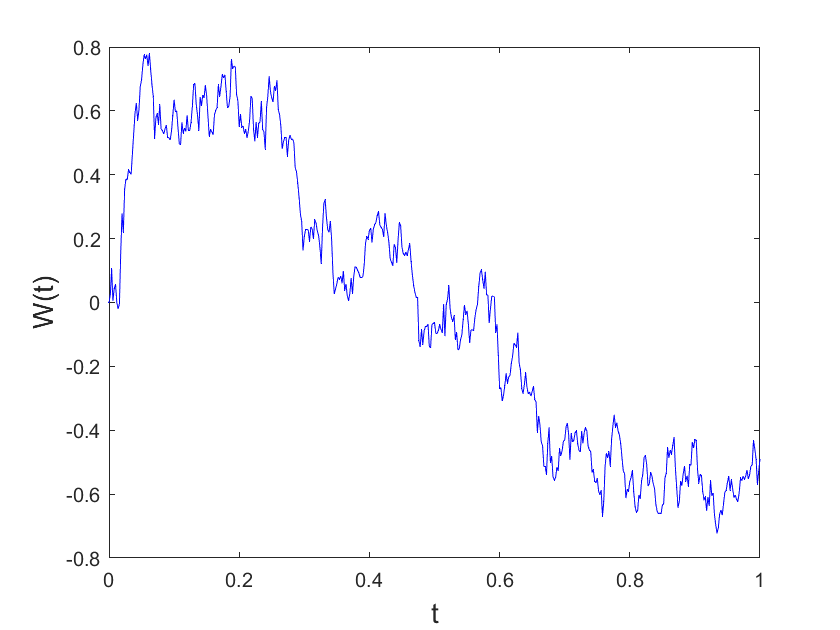
\includegraphics[width=0.9\textwidth]{graphics/single_brownian_motion.png}
                    \caption{Single Brownian Motion}
    \end{figure}
\newpage
\begin{lstlisting}[language=Matlab, caption={My MATLAB Code}, label={lst:matlabcode}]
Mc = 4;

for k=1:Mc
    T = 1;
    N = 1000;
    dt = T/N;
dW = zeros(1,N);
W = zeros(1,N); 
dW(1) = sqrt(dt)*randn;
W(1) = dW(1);
for j = 2:N
dW(j) = sqrt(dt)*randn; 
W(j) = W(j-1) + dW(j);
end
plot([0:dt:T],[0,W])
hold on;
end
xlabel('t','FontSize',10)
ylabel('W(t)','FontSize',10,'Rotation',90)

\end{lstlisting}
\newpage

 \begin{figure}[h]
      \centering
                    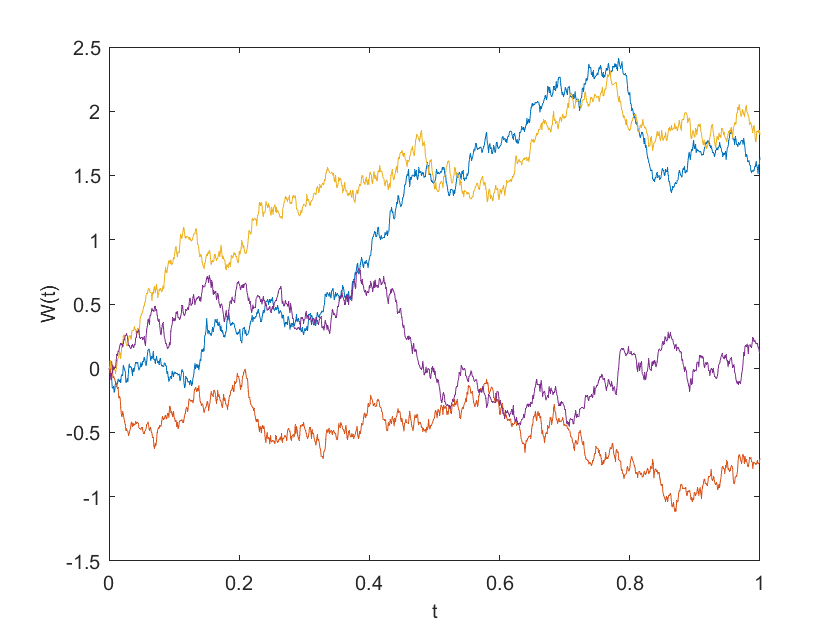
\includegraphics[width=0.9\textwidth]{graphics/plot_bm.png}
                    \caption{Multiple Brownian Motion}
    \end{figure}

\pagebreak

\subsection{Martingale}

    \textbf{Filtration:}\\
    Increasing family of sub $\sigma$-algebras $\{\mathcal{F}_t\}$ of $\mathcal{F}$\\
    $\mathcal{F}_0  \subseteq \mathcal{F}_s  \subseteq \mathcal{F}_t  \subseteq \mathcal{F}$ if $0 \leq s \leq t$\\
    \textbf{Right-Continuous:} \\ 
    A filtration is said to be right-continuous if 
    \[ \bigcap_{t > s} \mathcal{F}_t = \mathcal{F}_s\]

    A stochastic process $\{X_t\}_{t \geq 0}$ is called a Martingale with respect to a filtration if it satisfies
    \begin{itemize}
        \item ${E}[\left| X_t \right|] < \infty \ \forall \ t \geq 0$.
        \item $X_t$ is $\mathcal{F}_t$ measurable (adaptedness).
        \item ${E}[X_t|\mathcal{F}_s] = X_s, \ 0 \leq s \leq t$.
    \end{itemize}


\pagebreak

\section{Stochastic Integrals}

\subsection{Wiener Integral}
 \begin{itemize}
        \item Suppose $f$ is a step function given by $f = \sum_{i=1}^n a_i \cdot \mathbf{1}_{[t_{i-1}, t_i]}$, where $t_0 = 0$ and $t_n = T$. In this case, define 
        \[\mathbf{I}(f) = \int_0^{T}{f(t)\,dW_t} = \sum_{i=1}^n a_i \cdot (W(t_i) - W(t_{i-1}))\]
        where $f \in L^2[0,T]$ is a step process.

            \item Let $f \in L^2[0,T]$. The limit $\mathbf{I}(f) = \lim_{n \to \infty} \mathbf{I}(f_n)$ in $L^2(\Omega)$ is called the Wiener integral of $f$. The Wiener integral $\mathbf{I}(f)$ of $f$ will be denoted by:
\[ \mathbf{I}(f)(\omega) = \int_{0}^{T} f(t) \, dW(t)(\omega) \]
 where $f_n \in L^2[0,T]$ is a sequence of step process.
        \end{itemize}

\subsection{Properties of Wiener Integral}
$\mathbf{I}(f) = \int_0^T f(t)\,dW_t$ is a \textbf{Normal Random variable} with mean $0$ and variance $\int_0^T f(t)^{2}\,dt$.
\begin{enumerate}
    \item $E[\int_0^T f(t)\,dW_t] = 0$.
    \item $E[(\int_0^T f(t)\,dW_t)^{2}] = \int_0^T f^{2}(t)\,dt$.
    \item Let $f \in L^2[0,T]$.Then the stochastic process \[ M_t = \int_0^t f(s)\,dW(s),\ 0 \leq t \leq T,\] is a martingale with respect to $\mathcal{F}_t$, where $\mathcal{F}_t = \sigma\{W_s:0\leq s\leq t\}$.
\end{enumerate}
\subsection{\texorpdfstring{It$\hat{\text{o}}$ Integral}{Ito Integral}}

 \begin{itemize}
       \item Fix a Brownian motion $W(t)$ and filtration $\{ \mathcal{F}_t; \ 0 \leq t \leq T \}$ satisfying the following conditions:
       \begin{enumerate}
           \item For each $t$, $W(t)$ is $\mathcal{F}_t$-measurable.
           \item For any $s \leq t$, the random variable $W(t) - W(s)$ is independent of the $\sigma$-algebra $\mathcal{F}_s$.
       \end{enumerate}
       \item We will use $L_\text{ad}^2([0,T] \times \Omega)$ to denote the space of all stochastic process $f(t,\omega), \ 0 \leq t \leq T, \ \omega \in \Omega$ satisfying the following conditions:
       \begin{enumerate}
           \item $f(t,\omega)$ is adapted to the filtration $\{\mathcal{F}_t\}$.
           \item $\int_0^T{E({\left | f(t) \right |}^2)}\,dt < \infty$.
       \end{enumerate}
        \item \[f(t,\omega) = \sum_{i=1}^{n}{a_{i-1}(\omega)\mathbf{1}_{[t_{i-1},t_i]}(t)}\]
        \[\mathbf{I}(f) = \int_0^T f(t,\omega)\,dW_t(\omega) = \sum_{i=1}^n{a_{i-1}(W(t_i) - W(t_{i-1}))}\]
           \end{itemize}

\subsection{\texorpdfstring{Properties of It$\hat{\text{o}}$ Integral}{Properties of Ito Integral}}
  $f \in L_\text{ad}^2([0,T] \times \Omega)$. $\mathbf{I}(f) = \lim_{n \rightarrow \infty}\mathbf{I}(f_n)$ where $\{f_n(t,\omega); \ n \geq 1\}$ is a sequence of adapted step stochastic process.
        \begin{enumerate}
            \item ${E}[\int_0^T f(t)\,dW] = 0$.
          \item ${E}[(\int_0^T f(t)\,dW_t)^{2}] = E[\int_0^T f^{2}(t)\,dt]$ 
          \item If $f \in L^2_\text{ad}[(0,T) \times \Omega]$, then the indefinite integral $\mathbf{I}(\cdot)$ is a \textbf{Martingale}. Furthermore, $\mathbf{I}(\cdot)$ has a version with continuous sample paths a.s.
        \end{enumerate}

 


\subsection{\texorpdfstring{It$\hat{\text{o}}$ Formula}{Ito Formula}}
\begin{itemize}
     \item $X(\cdot)$ is a real-valued stochastic process satisfying \[ X(r) = X(s) + \int_s^r F\,dt + \int_s^r G\,dW\] for some $F \in L^1_\text{ad}[(0,T)\times \Omega], G \in L^2_\text{ad}[(0,T)\times \Omega]$ and all times $0 \leq  s \leq r \leq T$.We say that $X(\cdot)$ has the stochastic differential 
     \[ dX = F dt + G\,dW\] for $0 \leq t \leq T$
     \item $X(\cdot)$ has a stochastic differential \[ dX = F dt + G\,dW\] for $F \in L^1_\text{ad}[(0,T)\times \Omega], G \in L^2_\text{ad}[(0,T)\times \Omega]$.Assume $u \colon \mathbb{R} \times [0,T] \rightarrow \mathbb{R}, u = u(x,t)$ is continuous and that its partial derivatives $u_t = \frac{\partial u}{\partial t}, u_x = \frac{\partial u}{\partial x}$ and $u_{xx} = \frac{\partial^2 u}{\partial x^2}$  exist and are continuous.\\
     Then $Y(t) := u(X(t),t)$ has the stochastic differential 
     \begin{align*}
         \,du(X,t) &= u_t\,dt + u_x\,dX + \frac{1}{2} u_{xx} G^2\,dt\\
         &= (u_t + u_x F + \frac{1}{2} u_{xx} G^2)\,dt + u_x G\,dW
     \end{align*}
 \end{itemize}


\newpage
\section{Stochastic Differential Equations}

 \[dX(t) = f(t,X(t))\,dt + \sigma(t,X(t))\,dW_t, \quad t \in (0,T) \]  \[X(0) = X_0 \quad  \dots \text{ (1)} \] 
    \[X(t) = X_0 + \int_0^t f(s,X(s))\,ds + \int_0^t \sigma(s,X(s))\,dW_s \quad \text{almost surely in} \ P.\]
\subsection{Defination of SDE}
  A stochastic process $X \colon [0,T] \times \Omega \rightarrow \mathbb{R}$ is called a solution of the SDE (1) if
    \begin{itemize}
        \item $X(\cdot)$ is progressively measurable.(i.e. $X \colon [0,t] \times \Omega \rightarrow \mathbb{R} \text{ is } \mathcal{B}[0,t]\times\mathcal{F}_t$ measurable for all $t \geq 0$).
        \item $f(\cdot,X(\cdot)) \in L_{\text{ad}}^1([0,T] \times \Omega)$.
        \item $\sigma(\cdot,X(\cdot)) \in L_{\text{ad}}^2([0,T] \times \Omega)$.
        \item $\forall t \in [0,T],X(t)$ satisfies
        \[X(t) = X_0 + \int_0^t f(s,X(s))\,ds + \int_0^t \sigma(s,X(s))\,dW_s \quad \text{almost surely in} \ P.\]
    \end{itemize}



\subsection{Existence and Uniqueness Theorm}
   Let $f \colon [0,T] \times \mathbb{R} \rightarrow \mathbb{R}$ and $\sigma \colon [0,T] \times \mathbb{R} \rightarrow \mathbb{R}$ are continuous and for some $L > 0$ satisfies 
    \[ \left|f(t,x) - f(t,y)\right| \leq L\left|x-y\right|, \ \left|\sigma(t,x) - \sigma(t,y)\right| \leq L\left|x-y\right|\]
    \[ \left|f(t,x)\right| \leq L(1+\left|x\right|) ,\left|\sigma(t,x)\right| \leq L(1+\left|x\right|) \ \forall t \in [0,T], x \in \mathbb{R}\]
    Let $X_0 \colon \Omega \rightarrow \mathbb{R}$ be random variable, ${E}\left|X_0\right|^2 < \infty $. Then, there exists a unique solution $X \in L^2_\text{ad}([0,T] \times \Omega)$ of SDE(1).


\pagebreak
\section{Deterministic vs Stochastic Differential Equation}

\subsection{Euler's scheme to solve the ODE}

\[\frac{dy}{dt} = f(t,y(t)),\ 0 \leq t \leq T\]
      \[y(0) = y_0\]
      is given by:
      \[\omega_0 = y_0\]
      \[\omega_{n+1} = \omega_n + hf(t_n,\omega_n),\]
      \[n=0,1,\dots,N-1\] 
      where $h=\frac{T}{N}, \ t_n = nh$

      Now we may plot a graph by using this scheme.\\

      \textbf{For example}
      \begin{lstlisting}[language=Matlab, caption={My MATLAB Code}, label={lst:matlabcode}]
clc;
clear;
h = 0.02;
a = 0;
b = 1;
N = (b - a) / h;
w = zeros(1, N);
t = zeros(1, N);
t(1) = a;
w(1) = 1; % Initial value of y
for i = 2:N
    w(i) = w(i-1) + h * (cos(2*t(i-1)) + sin(3*t(i-1)));
    t(i) = a + i * h;
end
plot([a, t], [1, w], 'b-')
xlabel('t')
ylabel('y(t)')
title("Solution of y' = cos(2t) + sin(3t), y(0) = 1")

\end{lstlisting}
       \begin{figure}[h]
      \centering
                    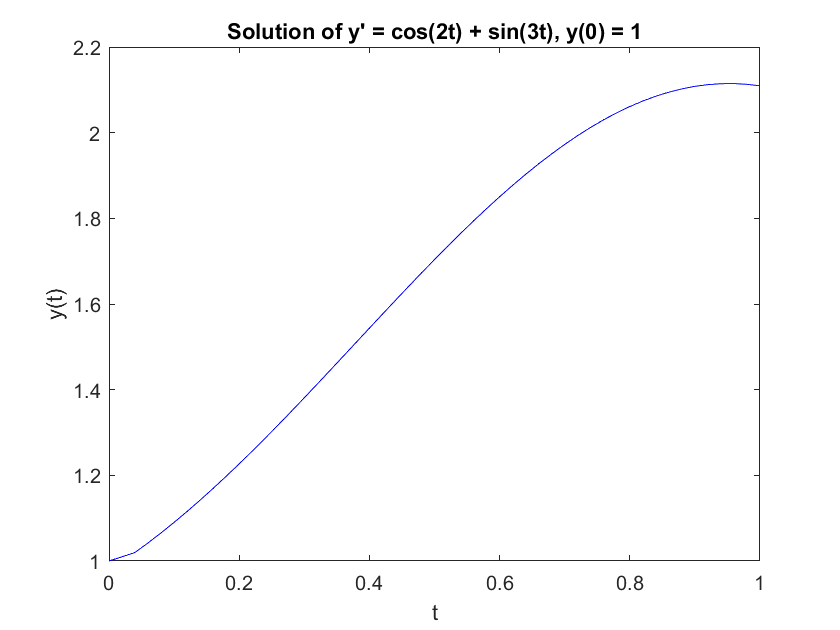
\includegraphics[width=0.8\textwidth]{graphics/eqn_4.png}
                    \caption{Deterministic Differential Equation}
\end{figure}
      


\subsection{Euler-Maruyama scheme to solve the SODE}

\[dX(t) = f(t,X(t))\,dt + \sigma(t,X(t))\,dW_t,\ 0 \leq t \leq T \]
      \[X(0) = X_0\]
      is given by:
      \[X_{n+1} = X_n + hf(t_n,X_n) + \sigma(t_n,X_n)\Delta dW_n,\]  \[n=0,1,\dots,N-1\]
      where $h=\frac{T}{N}, \ t_n = nh,$\\
      $ \Delta W_n = W(t_{n+1}) - W(t_n) \approx \sqrt{h}N(0,1)$
      Now we may plot a graph by using this scheme.\\

      \textbf{For example}
   \begin{lstlisting}[language=Matlab, caption={My MATLAB Code}, label={lst:matlabcode}]
  clc; 
clear;
Mc=2^4; %monte carlo samples
T = 1;
N = 2^6;
dt = T/N;
SW=0;
Sx = zeros(1,N+1);
Sx(1) = 1;
X = zeros(1,N+1);
X(1)=1;
mu = 1;
sigma = 0.1;
for k = 1:Mc
for n = 1:N   
    %X(n+1) = X(n) + dt*f(t(n),X(n)) + sigma(t(n),X(n))*sqrt(dt)*randn;
    X(n+1) = X(n) + mu*X(n)*dt + sigma*sqrt(dt)*randn;
    Sx(n+1) = Sx(n+1) + X(n+1);  
end
t=[0:dt:T];
hold on
plot(t,X);
end
%plot(t,S,LineWidth=4,Color='r');
S = Sx /Mc;
S(1) = X(1);
plot(t,S,LineWidth=2,Color='r');
legend('Monte Carlo Paths');
lineHandle = findobj('Type', 'line', 'LineWidth', 2);
legend(lineHandle, 'E(X)');
xlabel('t')
ylabel('X(t)')
title("dX(t) = X(t)dt + 0.1sqrt(t)dW(t), X(0) = 0")
hold off

\end{lstlisting}   


\begin{figure}[h]
      \centering
                    \includegraphics[width=0.8\textwidth]{graphics/eqn_10.png}
                    \caption{Stochastic differential equation}
    \end{figure}
    
\pagebreak
\subsection{Comparison}
We can compare two identical equations: one that includes a stochastic (random) term, and the other that only contains deterministic terms.\\
(a) $\,dy(t) = (t^2 + y^2)\,dt$, $y(0) = 0$\\
(b) $\,dX(t) = (t^2 + X^2)\,dt + tX(t)\,dW(t)$, $X(0) = 0$\\


Now that we have graphs for both of these equations, we can compare them:
\begin{lstlisting}[language=Matlab, caption={My MATLAB Code}, label={lst:matlabcode}]
clc;
clear;
h = 0.02;
a = 0;
b = 1;
N = (b - a) / h;
w = zeros(1, N);
t = zeros(1, N);
t(1) = a;
w(1) = 0; % Initial value of y
for i = 2:N
    w(i) = w(i-1) + h * (t(i-1)^2 + w(i-1)^2);
    t(i) = a + i * h;
end
plot([a, t], [0, w], 'b-',LineWidth=2)
ylim([0, 0.6]);
xlabel('t')
ylabel('y(t)')
title("y' = t^2 + y^2, y(0) = 0")

\end{lstlisting}
\newpage
\begin{lstlisting}[language=Matlab, caption={My MATLAB Code}, label={lst:matlabcode}]
clc;
clear;
Mc=2^4; %monte carlo samples
T = 1;
N = 2^6;
dt = T/N;
Sw = zeros(1,N+1);
f = @(t,x) t^2 + x^2; % f = inline('t^2 + x^2');
sig = @(t,x) t*x; % sig = inline ('t*x');
t=[0:dt:T];
X = zeros(1,N+1);
X(1)=0;
for k = 1:Mc
for n = 1:N
    X(n+1) = X(n) + dt*f(t(n),X(n)) + sig(t(n),X(n))*sqrt(dt)*randn;    
    Sw(n+1) = Sw(n+1) + X(n+1);   
end
plot(t,X);
hold on
end
S = Sw./Mc;
S(1) = X(1);
plot(t, S, 'LineWidth', 2, 'color', 'r');
% Create a legend entry only for the line with width 2
legend('Monte Carlo Paths');
lineHandle = findobj('Type', 'line', 'LineWidth', 2);
legend(lineHandle, 'E(X)');
hold off
xlabel('t')
ylabel('X(t)')
title("dX(t) = (t^2 + X^2)dt + tX(t)dW(t), X(0) = 0")



\end{lstlisting}
\newpage
 \begin{figure}[h]
      \centering
                    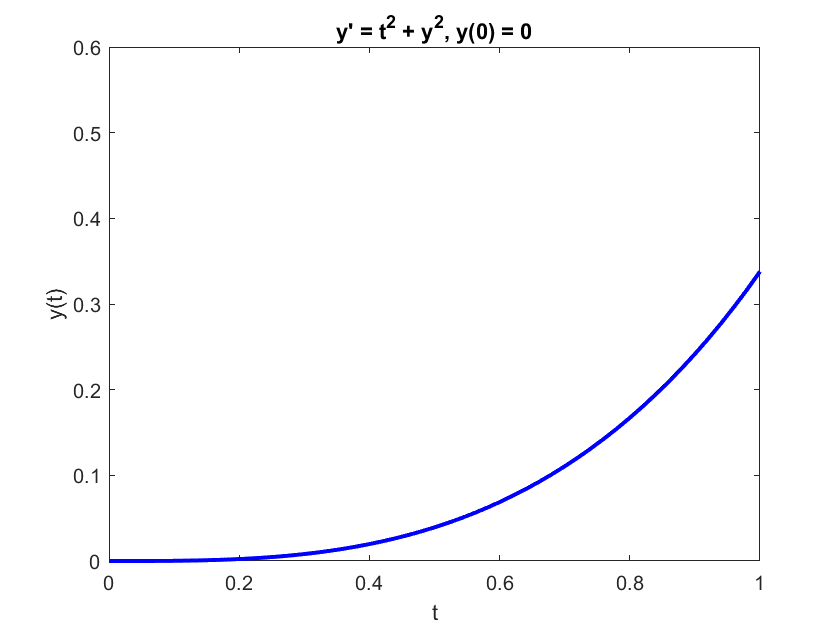
\includegraphics[width=0.8\textwidth]{graphics/deterministic_SDE.png}
                    \caption{(a) ODE}
    \end{figure}
    \newpage
     \begin{figure}[h]
      \centering
                    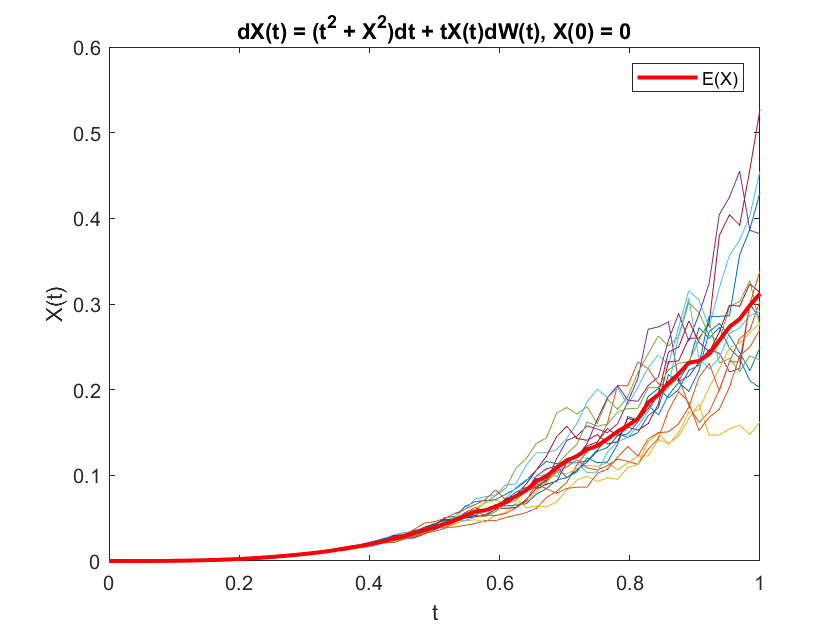
\includegraphics[width=0.8\textwidth]{graphics/stochastic_SDE.png}
                    \caption{(b) SODE}
    \end{figure}




\newpage
\section{Examples}

        \subsection{Stock Price}
        Let $S(t)$ denote the stock prices at time $t$. The evolution of $S(t)$ is given by the SDE: 
        \[\frac{d S(t)}{S(t)} = \mu\,dt + \sigma\,dW_t\]
        \[t > 0, \ S(0) = S_0, \ \mu > 0, \ \sigma \in \mathbb{R}\]
        where $\mu$ is drift and $\sigma$ is volatility.
        As above differential equation is the same as in the example-(32). So, solution of this SDE is in form of $S(t) = S_0 e^{Y(t)}$\\
$dY(t) = \mu.dt + \sigma.dW_t - \frac{1}{2} \sigma^2.dt$
\begin{align*}
    Y(t) &= \int_0^t \mu.ds + \int_0^t \sigma.dW_s - \frac{1}{2} \int_0^t \sigma^2.ds\\
    Y(t) &= \mu t + \sigma W_t - \frac{1}{2} \sigma^2 t  
\end{align*} 
$\therefore S(t) = S_0 e^{ (\mu t + \sigma W_t - \frac{1}{2} \sigma^2 t)}\\
dS(t) = \mu S(t).dt + \sigma S(t).dW_t \Leftrightarrow
S(t) = S_0 + \int_0^t \mu S(s).ds + \int_0^t \sigma S(s).dW_s $

 Finding expectation of $S(t)$
\begin{align*}
    {E}[S(t)] &= S_0 +  \mu {E}[\int_0^t S(s).ds] + \sigma {E}[\int_0^t S(s).dW_s] \\
    &= S_0 +  \mu {E}[\int_0^t S(s).ds] \\
    &= S_0 + \mu \int_0^t {E}[S(s).ds] \ \text{Using Fubini theorem}
    \text{Let ${E}[S(t)] = m(t)$}\\
    m(t) &= m_0 + \mu \int_0^t m(s).ds\\
    \text{differential the above equation}\\
    \frac{d m(t)}{dt} &= \mu m(t) \\
    \text{On integrating }\\
    m(t) &= m_0 e^{\mu t}\\
    {E}[S(t)] &= {E}[S_0] e^{\mu t} \\
    &= S_0 e^{\mu t} \text{(if $S_0$ is determinate)}
\end{align*}
  \[ S(t) = S_0 e^{[(\mu - \frac{1}{2}\sigma^2)t +\sigma W_t]} \]
  \newpage
        \subsection{Brownian Bridge}
        \[dB(t) = \frac{-B}{1-t}\,dt + \,dW_t\]
        \[0 < t < 1,\ B(0) = 0\]
    By using Euler-Maruyama Scheme, we may plot the graph for as many samples for Brownian Bridge and then take the expected line for the same.
        \begin{lstlisting}[language=Matlab, caption={My MATLAB Code}, label={lst:matlabcode}]
clc;
clear;
Mc=2^4; %monte carlo samples
T = 1;
N = 2^6;
dt = T/N;
Sw = zeros(1,N+1);
f = @(t,B) B/(t-1); % f = inline('B/(t-1)');
sig = @(t,B) 1; % sig = inline ('1');
t=[0:dt:T];
B = zeros(1,N+1);
B(1)=0;
for k = 1:Mc
for n = 1:N
    B(n+1) = B(n) + dt*f(t(n),B(n)) + sig(t(n),B(n))*sqrt(dt)*randn;  
    Sw(n+1) = Sw(n+1) + B(n+1);   
end
plot(t,B);
hold on
end
S = Sw./Mc;
S(1) = B(1);
plot(t, S, 'LineWidth', 2, 'color', 'r');
% Create a legend entry only for the line with width 2
legend('Monte Carlo Paths');
lineHandle = findobj('Type', 'line', 'LineWidth', 2);
legend(lineHandle, 'E(B)');
hold off
xlabel('t')
ylabel('B(t)')
title("dB(t) = (B/(t-1))dt + dW(t), B(0) = 0")


\end{lstlisting}

\begin{figure}[h]
      \centering
                    \includegraphics[width=0.8\textwidth]{graphics/bm_bridge.png}
                    \caption{Brownian Bridge}
\end{figure}
        \subsection{Langevin's Equation}
        \[\,dX(t) = -bX(t)\,dt + \sigma\,dW_t\]
        \[t > 0 , \ X(0) = X_0\]

\pagebreak
\section{Conclusion}

In conclusion, the research project on Stochastic Differential Equations (SDEs) has provided a comprehensive exploration of the fundamental concepts, properties, and applications of this mathematical framework. Through the study of probability spaces, random variables, and stochastic processes, the project has established the mathematical foundations necessary for understanding SDEs.

The project has highlighted the importance of SDEs in modeling dynamic systems affected by random fluctuations. The investigation of stochastic integrals and numerical approximation schemes has equipped researchers with practical tools for solving SDEs and approximating their solutions.

Furthermore, the project has showcased the practical applications of SDEs in finance, where they are widely used to model stock prices and options pricing. This demonstrates the significant impact of SDEs in capturing uncertainties and complex dynamics within financial markets.

By bridging theory and application, this project has deepened our understanding of SDEs and their relevance in various scientific disciplines. The insights gained have far-reaching implications, enabling more accurate predictions, risk assessments, and informed decision-making in fields influenced by random dynamics.

Overall, the research project on Stochastic Differential Equations has contributed to our knowledge and appreciation of these mathematical tools. As researchers continue to explore their applications and refine the theory, SDEs will remain invaluable in modeling and analyzing complex systems subject to random fluctuations.

\pagebreak
\section{References}

 \begin{itemize}
        \item \href{https://drive.google.com/file/d/1vRMD3PfWG5iZTjwdAeLyz3_fwPLslEyn/view?usp=drive_link}{Kuo H. H.,-Introduction to Stochastic Integration-Springer (2005)}
        \item \href{https://drive.google.com/file/d/1dDVWcERBHMOOmIBrovXGwt5KPLrIyRxC/view?usp=drive_link}{Oksendal B-Stochastic Differential Equations-Springer (2000)}
        \item \href{https://drive.google.com/file/d/1EiN6uab1nWAKvLPzE0VfQuoJ4vpF1bjM/view?usp=drive_link}{Evans L. C. - An Introduction to Stochastic Differential Equations (2014)}
        \item \href{https://drive.google.com/file/d/1xmvYTdusN2AgJ88izdlyRi1nP0L7RGdY/view?usp=drive_link}{Xuerong Mao-Stochastic Differential Equations and Applications-Woodhead Publishing(2011)}
        \item \href{https://drive.google.com/file/d/1pPIpvQBrxkK69bebNpvoupaZNODOAGIk/view?usp=drive_link}{Siva Athreya, V. S. Sunder - Measure and Probability-CRC Press (2008)}
    \item \href{https://www.dropbox.com/scl/fo/o18jjmcgnvwu23ye2wwba/h?dl=0&rlkey=0n9ibd9u21w8oykfg7hut3hyf}{Athreya and Lahiri -Measure and Probability Theory (2006)}
        
    \end{itemize}

\clearpage




\end{document}
